\documentclass{beamer}

\usepackage[utf8]{inputenc} \usepackage{bibentry,cite,amsmath,graphicx}

\newcommand{\Z}{\mathbb{Z}} \newcommand{\N}{\mathbb{N}}
\newcommand{\R}{\mathbb{R}} \newcommand{\E}{\operatorname{E}}
\newcommand{\Var}{\operatorname{Var}} \newcommand{\Cov}{\operatorname{Cov}}
\newtheorem{proposition}{proposition}
% Information to be included in the title page:
\title{The Extended Kalman-Bucy Filter} \author{Alexander Wittmond} \institute{University of
  Missouri} \date{\today}

\AtBeginSection[] {
  \begin{frame}
    \frametitle{Table of Contents}
    \tableofcontents[currentsection]
  \end{frame}
}

\usetheme{Hannover} \allowdisplaybreaks
\begin{document}

\frame{\titlepage}


\begin{frame}{Extension to Non-Linear Problems}
  We start with the system
  \begin{align}
    dx_t = f(x_t,t)dt + G(t)d\beta_t \\
    y_k = h(x_{t_k}, t) + \nu_t
  \end{align}
  where
  \begin{equation}
    \mathbb{E}[d\beta_td\beta^T_t] = Q(t) dt
  \end{equation}
  \pause
  Then we pick a \textbf{reference trajectory} $\bar{x}_{t_0}(t)$ with some given
  $\bar{x}(t_0)$ such that
  \begin{equation}
    \frac{d\bar{x}_{t_0}}{dt}(t) = f(\bar{x}_{t_0}(t),t)
  \end{equation}
\end{frame}

\begin{frame}{Extension to Non-Linear Problems}
  Then we can look at the \textbf{deviation}
  \begin{equation}
    \delta x(t) = x(t) - \bar{x}_{t_0}(t) 
  \end{equation}
  which statisfies
  \pause
  \begin{equation}
    d(\delta x_t) = (f(x_t,t) - f(\bar{x}_{t_0}(t),t)) dt + G(t) d\beta_t
  \end{equation}
  \pause
  then do a Taylor approximation
  \begin{equation}
    f(x_t,t) - f(\bar{x}_t,t) \simeq Df(\bar{x}_{t_0}(t),t)  \delta x_t 
  \end{equation}
  \pause
  Then we have the linear equation
  \begin{equation}
    d(\delta x_t) = Df(\bar{x}_{t_0} , t) \delta x_t dt + G(t) d\beta_t
  \end{equation}
\end{frame}

\begin{frame}{Extension to Non-Linear Problems}
  We can linearize the measurement in the same way to get
  \begin{align}
    \delta y_{t_k} &= y_{t_k} - h(\bar{x}_{t_0}(t_k), t_k) + \nu_k \\
    \delta y_{t_k} &\simeq Dh(\bar{x}_{t_0}(t_k),t_k) \delta x_{t_k} + \nu_k
  \end{align}
  \pause
  Then we can process the system
  \begin{align}
    d(\delta x_t) &= Df(\bar{x}_{t_0}(t),t) \delta x_t dt + G(t) d\beta_t \\
    \delta y_{t_k} & = Dh(\bar{x}_{t_0}(t_k),t_k) \delta x_{t_k} + \nu_k
  \end{align}
  with  linear filter.
\end{frame}

\begin{frame}{Extension to Non-Linear Problems}
  We can then estimate $\hat{x}_{t_k}^{t_k}$ with
  \begin{align}
    \hat{x}_{t_k}^{t_k} = \bar{x}_{t_0}(t_k) + \hat{\delta x_{t_k}^{t_k}}
  \end{align}
  Our variance matrix $P_{t_k}^{t_k}$ estimates the variance of this
  estimation.
\end{frame}

\begin{frame}{Extension to Non-Linear Problems}
  If at every observation $h(t_k)$, we relinearize around our estimate
  $\hat{x}_{t_k}^{t_k}$ by getting a new reference trajectory $\bar{x}_{t_k}(t)$
  starting at this point, and then estimate the system using

  
  \begin{align}
    d(\delta x_t) &= Df(\bar{x}_{t_k}(t),t_k) \delta x_t dt + G(t) d\beta_t \\
    \delta y_{t_{k+1}} &\simeq Dh(\bar{x}_{t_k}(t_k),t_k) \delta x_{t_k} + \nu_k
  \end{align}

  then this is known as the \textbf{Extended Kalman Filter}
\end{frame}

\begin{frame}{In Code}

\begin{figure}
  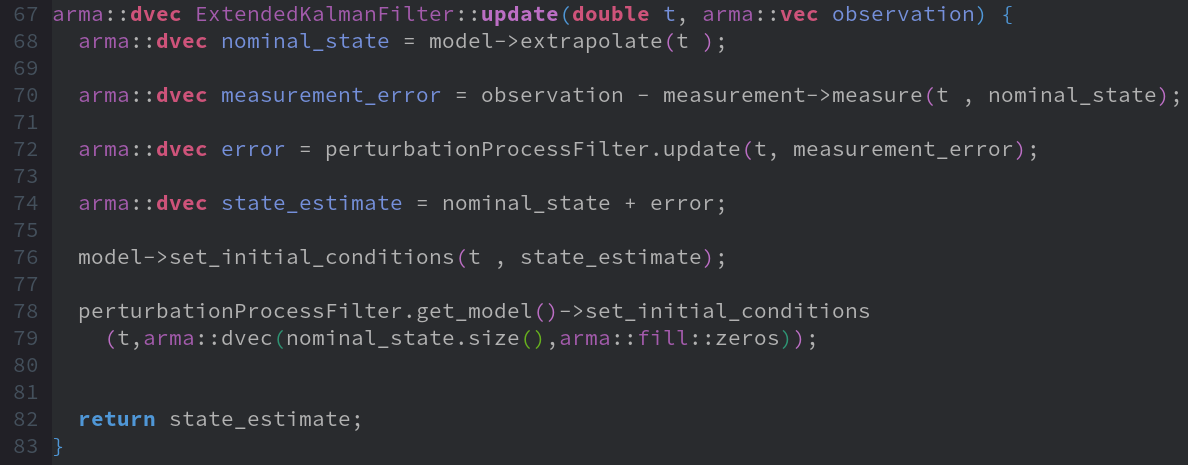
\includegraphics[scale=0.3]{ekf_implementation.png}
  \caption{The Extended Kalman Filter update in C++}

\end{figure}
\end{frame}

\begin{frame}{Pros and Cons}
  \begin{box}{Pros}
    \begin{itemize}
   \pause  
    \item Recursiveness causes low memory requirements
   \pause  
    \item Relatively low cost to computing an update
   \pause  
    \item Most computationally expensive items can be computed in advance

    \end{itemize}
  \end{box}
\pause
  \begin{box}{Cons}
    \begin{itemize}
\pause
    \item  Is not adaptive, relies on the accuracy of the underlying model
\pause

  \item  Suffers from filter divergence

  \pause 

    \item  Can not capture multi-modalities
    \end{itemize}

  \end{box}
\end{frame}
  

\end{document}
